\chapter{Objetivos}
\label{cap:capitulo2}

\vspace{1cm}

En este capítulo se describe el problema abordado, así como los objetivos que se quieren lograr, después de haber presentado el contexto y el estado del arte en el que está ubicado este trabajo final de grado. De igual forma, se definen los requisitos del sistema propuesto, las competencias empleadas y adquiridas durante el desarrollo del proyecto, la metodología seguida y el plan de trabajo llevado a cabo.\\

\section{Descripción del problema}
\label{sec:descripcion}

La administración adecuada de la medicación y el monitoreo de parámetros fisiológicos básicos representan un reto importante en el contexto de la asistencia sanitaria a domicilio, sobre todo en pacientes crónicos o ancianos. Los sistemas existentes suelen presentar un coste elevado o una complejidad de uso que dificulta su adopción en entornos domésticos. Esto puede resultar en errores al tomar medicamentos o en una inadecuada supervisión de la salud del paciente. En este contexto, resulta de interés el desarrollo de soluciones accesibles y de bajo coste que posibiliten automatizar estas tareas, facilitando la autonomía del usuario y mejorando la seguridad en el seguimiento de los tratamientos.\\

Con esta finalidad, el objetivo principal del presente trabajo es la creación y elaboración de un sistema robótico de bajo coste, orientado a la asistencia sanitaria en el hogar, basado en sensores, un microcontrolador con pantalla táctil y una aplicación móvil de supervisión. El sistema propuesto se compone de un pastillero automatizado que puede manejar la gestión de medicamentos a través de alertas acústicas y visuales, además de registrar parámetros fisiológicos como la saturación de oxígeno en sangre y el ritmo cardíaco.\\

Para alcanzar este objetivo general, se plantean los siguientes subobjetivos:

\begin{enumerate}
    \item Diseñar la arquitectura general del sistema, definiendo los componentes hardware y software necesarios para su funcionamiento.

    \item Desarrollar el diseño mecánico del pastillero automatizado mediante herramientas de modelado 3D, permitiendo su fabricación mediante impresión 3D con materiales de bajo coste.

    \item Seleccionar e integrar el microcontrolador, así como implementar la lógica de control del sistema para la gestión de sensores, actuadores y avisos.

    \item Diseñar e implementar una interfaz de usuario basada en pantalla táctil que permita interactuar con el dispositivo de forma sencilla e intuitiva.

    \item Integrar un sensor biomédico capaz de medir la frecuencia cardiaca y la saturación de oxígeno en sangre, permitiendo registrar estos datos.

    \item Desarrollar una aplicación móvil que permita configurar los horarios de medicación y consultar la información registrada por el sistema.

    \item Implementar un sistema de comunicación inalámbrica mediante WiFi entre el dispositivo y la aplicación móvil, incluyendo el intercambio y almacenamiento de datos.

    \item Realizar pruebas funcionales del sistema completo para verificar su correcto funcionamiento y evaluar su viabilidad como solución de bajo coste.
\end{enumerate}

\section{Requisitos}
\label{sec:requisitos}

Con el fin de cumplir los objetivos propuestos, se han establecido los siguientes requisitos técnicos que el sistema deberá satisfacer durante el desarrollo del proyecto:

\begin{enumerate}
\item El sistema deberá estar basado en un microcontrolador ESP32-2432S028, encargado de gestionar la interfaz de usuario, la comunicación y la lectura de sensores.

\item El software del dispositivo deberá desarrollarse en lenguaje C++, mientras que la aplicación móvil se implementará en Android Studio utilizando Kotlin.

\item La comunicación entre el dispositivo y la aplicación móvil deberá realizarse mediante conexión WiFi, garantizando un intercambio de datos fiable.

\item El sistema deberá ser capaz de funcionar en tiempo real, permitiendo la correcta gestión de avisos, lectura de sensores y actualización de información sin retardos perceptibles.

\item El diseño mecánico del dispositivo deberá realizarse mediante modelado 3D, de forma que las piezas puedan fabricarse mediante impresión 3D utilizando material PLA.

\item El coste total del prototipo deberá mantenerse dentro de un rango reducido, no superando los {50} \euro\  aproximadamente, con el fin de garantizar su accesibilidad.

\item El sistema deberá permitir el almacenamiento de datos relacionados con las tomas de medicación y las mediciones fisiológicas, accesibles desde la aplicación móvil.

\item El dispositivo deberá incorporar avisos visuales y acústicos que faciliten la correcta administración de la medicación.
\end{enumerate}

\section{Competencias}
\label{sec:competencias}

\subsection{Competencias empleadas}

Las competencias empleadas para la realización de este trabajo fin de grado, y que han sido adquiridas a lo largo del Grado en Ingeniería Robótica, son las siguientes:

\begin{enumerate}
    \item \textbf{CG02.} Capacidad de resolver problemas con iniciativa, toma de decisiones, creatividad, y de comunicar y transmitir conocimientos, habilidades y destrezas, comprendiendo la responsabilidad ética y profesional de la actividad de la Ingeniería Robótica. Ha sido necesaria para el diseño del sistema y la resolución de los distintos retos técnicos planteados durante el desarrollo.

    \item \textbf{CE06.} Capacidad para resolver problemas propios de la Ingeniería Robótica por medio de la programación de aplicaciones robustas, eficientes y seguras, aplicando técnicas algorítmicas adecuadas. Aplicada en el desarrollo del software del microcontrolador y de la aplicación móvil.

    \item \textbf{CE10.} Capacidad de diseñar y programar sistemas en red aplicando conceptos de arquitectura de red, protocolos e interfaces de comunicaciones. Utilizada en la implementación de la comunicación WiFi entre el dispositivo y la aplicación móvil.

    \item \textbf{CE12.} Capacidad de diseñar robots y sistemas inteligentes atendiendo a los elementos de sensorización y actuación más adecuados dependiendo de la aplicación, los requerimientos del sistema y las condiciones del entorno. Aplicada en la selección e integración de sensores biomédicos y elementos del sistema.

    \item \textbf{CE24.} Capacidad de programar y desplegar aplicaciones en microcontroladores y procesadores no convencionales atendiendo a sus características y los recursos disponibles. Fundamental en la implementación del sistema sobre el ESP32.

    \item \textbf{CE29.} Capacidad de diseñar robots y sistemas inteligentes orientados a la interacción con personas, y adaptados a entornos domésticos y urbanos. Aplicada en el diseño de la interfaz y la adaptación del sistema al entorno doméstico.
\end{enumerate}

\subsection{Competencias adquiridas}

Las competencias adquiridas con el desarrollo del presente trabajo fin de grado son las siguientes:

\begin{enumerate}
    \item \textbf{CB2.} Que los estudiantes sepan aplicar sus conocimientos a su trabajo o vocación de una forma profesional y posean las competencias que suelen demostrarse por medio de la elaboración y defensa de argumentos y la resolución de problemas dentro de su área de estudio. Esta competencia se adquiere mediante la aplicación práctica de los conocimientos desarrollados a lo largo del grado en la resolución del problema planteado.

    \item \textbf{CB4.} Que los estudiantes puedan transmitir información, ideas, problemas y soluciones a un público tanto especializado como no especializado. Se adquiere mediante la redacción de la memoria y la explicación del sistema desarrollado.

    \item \textbf{CB5.} Que los estudiantes hayan desarrollado aquellas habilidades de aprendizaje necesarias para emprender estudios posteriores con un alto grado de autonomía. Se adquiere mediante el desarrollo autónomo del proyecto, la investigación y la resolución de problemas.

    \item \textbf{CE32.} Desarrollo de las capacidades adecuadas para realizar un ejercicio original individual, presentarlo y defenderlo ante un tribunal universitario, consistente en un proyecto en el ámbito de las tecnologías específicas del campo de la Robótica. Esta competencia se cumple con la realización completa del presente trabajo fin de grado.
\end{enumerate}
 
\section{Metodología}
\label{sec:metodologia}

Para el desarrollo de este trabajo se ha seguido una metodología basada en el diseño e implementación progresiva del sistema. En una primera fase, se llevó a cabo el análisis del problema y de las tecnologías necesarias, lo que permitió definir la arquitectura del sistema y seleccionar los componentes hardware y software más adecuados. A partir de este punto, se desarrollaron de forma paralela los distintos módulos, incluyendo el diseño del dispositivo, la programación del microcontrolador, la integración de sensores y el desarrollo de la aplicación móvil, realizando pruebas parciales para validar cada componente.\\

\begin{figure}[H]
    \centering
    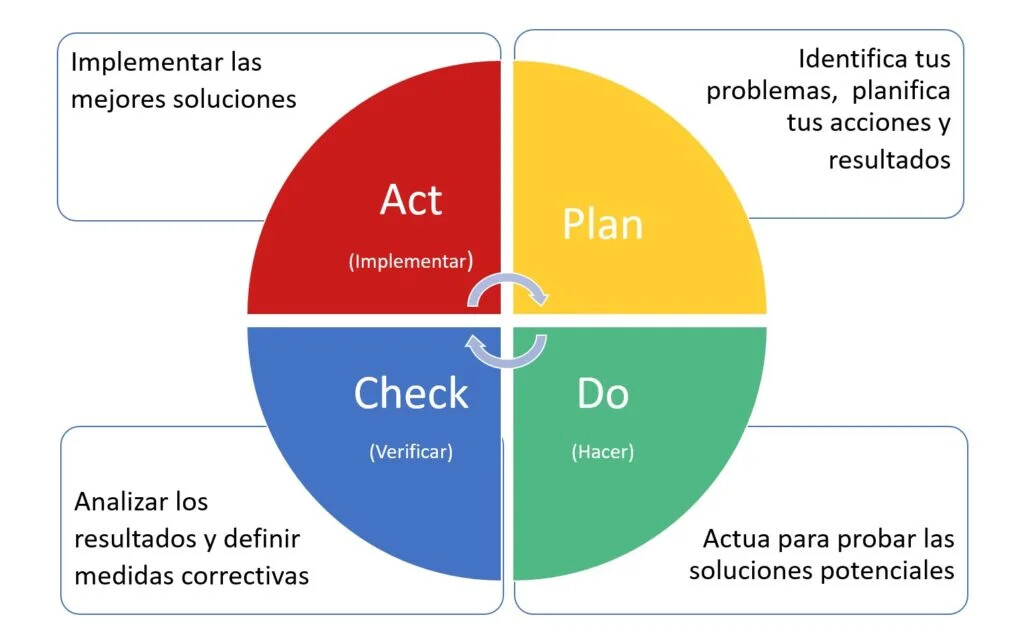
\includegraphics[width=0.85\textwidth]{figs/PDCA_esquema.jpg}
    \caption{Ciclo de mejora continua Plan--Do--Check--Act (PDCA)}
    \label{fig:PDCA}
\end{figure}

El proceso de desarrollo se ha apoyado en un enfoque iterativo basado en el ciclo Plan–Do–Check–Act (PDCA), representado en la Figura~\ref{fig:PDCA}, que ha permitido la mejora continua del sistema mediante la implementación, verificación y optimización de sus funcionalidades. Este enfoque se ha complementado con reuniones periódicas con el tutor, generalmente con una frecuencia semanal, en las que se han revisado los avances, resuelto dudas y definido nuevos objetivos. El trabajo se ha basado en la consecución de objetivos parciales y en la mejora progresiva del sistema, permitiendo alcanzar una solución final completa y funcional.\\

\section{Plan de trabajo}
\label{sec:plantrabajo}

El desarrollo del presente trabajo fin de grado se ha dividido en las siguientes etapas:

\begin{enumerate}
    \item \textbf{Investigación inicial:} Estudio del estado del arte y de las tecnologías necesarias para el desarrollo del sistema, incluyendo microcontroladores, sensores biomédicos y aplicaciones móviles.

    \item \textbf{Definición del sistema:} Diseño de la arquitectura general y selección de los componentes hardware y software adecuados.

    \item \textbf{Diseño del dispositivo:} Modelado 3D del pastillero automatizado y preparación de las piezas para su fabricación mediante impresión 3D.

    \item \textbf{Desarrollo del sistema:} Implementación del sistema, incluyendo la programación del microcontrolador, la integración de sensores y el desarrollo de la interfaz de usuario y la aplicación móvil.

    \item \textbf{Integración:} Conexión de los distintos módulos desarrollados, asegurando la correcta comunicación entre el dispositivo y la aplicación móvil.

    \item \textbf{Pruebas y validación:} Realización de pruebas funcionales para verificar el correcto funcionamiento del sistema y detectar posibles mejoras.

    \item \textbf{Redacción de la memoria:} Documentación del proceso seguido y de los resultados obtenidos.
\end{enumerate}

Todo el contenido del proyecto se encuentra disponible en un repositorio público de GitHub\footnote{\url{https://github.com/RoboticsURJC/tfg-amartinez}}, donde se incluye el código desarrollado y los recursos empleados durante la realización del trabajo. Además, en la wiki del repositorio se recoge de forma detallada el desarrollo del proyecto; en esta se han ido documentando de forma progresiva las distintas etapas, las decisiones tomadas y los avances realizados a lo largo del proyecto.\\

\

Tras haber definido los objetivos, requisitos, competencias, metodología y plan de trabajo del proyecto, en el siguiente capítulo se detallan las herramientas, tecnologías y plataformas empleadas para el desarrollo del sistema.
